\tikzset{every picture/.style={line width=0.75pt}} %set default line width to 0.75pt        

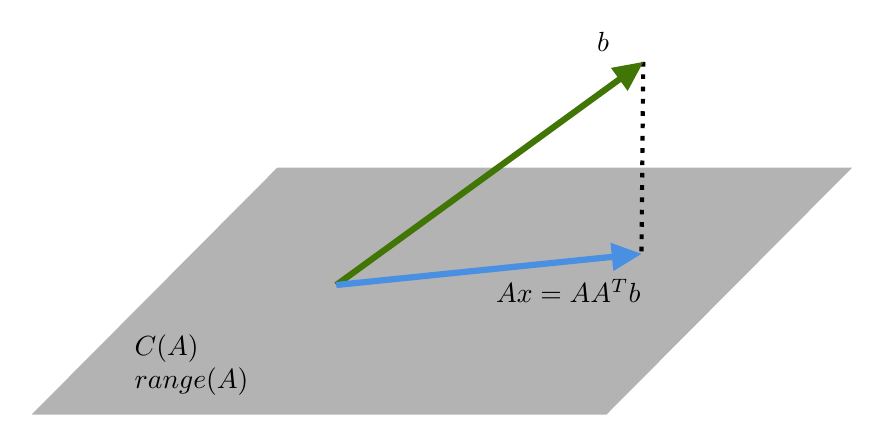
\begin{tikzpicture}[x=0.75pt,y=0.75pt,yscale=-1,xscale=1]
%uncomment if require: \path (0,300); %set diagram left start at 0, and has height of 300

%Shape: Parallelogram [id:dp5765772576295551] 
\draw  [color={rgb, 255:red, 255; green, 255; blue, 255 }  ,draw opacity=1 ][fill={rgb, 255:red, 179; green, 179; blue, 179 }  ,fill opacity=1 ] (203.26,170) -- (481.86,170) -- (362.46,290) -- (83.86,290) -- cycle ;
%Straight Lines [id:da4794253301098559] 
\draw [color={rgb, 255:red, 0; green, 0; blue, 0 }  ,draw opacity=1 ][line width=1.5]  [dash pattern={on 1.69pt off 2.76pt}]  (379.96,119.55) -- (379.07,212) ;
%Straight Lines [id:da5251055282063475] 
\draw [color={rgb, 255:red, 65; green, 117; blue, 5 }  ,draw opacity=1 ][line width=2.25]    (232.07,227) -- (375.92,122.49) ;
\draw [shift={(379.96,119.55)}, rotate = 504] [fill={rgb, 255:red, 65; green, 117; blue, 5 }  ,fill opacity=1 ][line width=0.08]  [draw opacity=0] (14.29,-6.86) -- (0,0) -- (14.29,6.86) -- cycle    ;
%Straight Lines [id:da14492521891839827] 
\draw [color={rgb, 255:red, 74; green, 144; blue, 226 }  ,draw opacity=1 ][line width=2.25]    (232.07,227) -- (374.09,212.51) ;
\draw [shift={(379.07,212)}, rotate = 534.1700000000001] [fill={rgb, 255:red, 74; green, 144; blue, 226 }  ,fill opacity=1 ][line width=0.08]  [draw opacity=0] (14.29,-6.86) -- (0,0) -- (14.29,6.86) -- cycle    ;

% Text Node
\draw (126.72,248.11) node [anchor=north west][inner sep=0.75pt]    {$ \begin{array}{l}
C( A)\\
\operatorname{range}( A)
\end{array}$};
% Text Node
\draw (356.21,103.52) node [anchor=north west][inner sep=0.75pt]    {$b$};
% Text Node
\draw (307.57,222.9) node [anchor=north west][inner sep=0.75pt]    {$Ax=AA^{T} b$};


\end{tikzpicture}